\documentclass[t]{beamer}
\usetheme{Copenhagen}
\setbeamertemplate{headline}{} % remove toc from headers
\beamertemplatenavigationsymbolsempty

\usepackage{amsmath, array, tikz, bm, pgfplots, tcolorbox, graphicx, venndiagram, color, colortbl, xfrac}
\pgfplotsset{compat = 1.16}
\usepgfplotslibrary{statistics}
\usetikzlibrary{calc}

\title{Discrete Probability Distributions}
\author{}
\date{}

\AtBeginSection[]
{
  \begin{frame}
    \frametitle{Objectives}
    \tableofcontents[currentsection]
  \end{frame}
}

\begin{document}

\begin{frame} 
\maketitle
\end{frame}

\section{Create a probability distribution}

\begin{frame}{Probability Distributions}
\begin{tcolorbox}[colframe=green!20!black, colback = green!30!white,title=\textbf{Probability Distribution}]
A \textbf{probability distribution} is a listing of each outcome of a probability experiment with their probabilities.
\end{tcolorbox}
\vspace{10pt} 

\onslide<2->{A {\color{blue}\textbf{discrete probability distribution}} is one in which the outcomes of each experiment are discrete (countable) values.}	\newline\\

\onslide<3->{Familiar Characteristics:}
\begin{itemize}
	\item<4-> $0 \leq \text{ each probability } \leq 1$
	\item<5-> The sum of all probabilities in a distribution equals 1
	\item<6-> $P(A \text{ or } B) = P(A) + P(B)$
\end{itemize}
\end{frame}

\begin{frame}{Probability Distribution of Rolling 2 Dice}
\begin{center}
\begin{tabular}{c|cccccc}
			&	\textbf{1}	&	\textbf{2}	&	\textbf{3}	&	\textbf{4}	&	\textbf{5}	&	\textbf{6}	\\	\hline
\textbf{1}	&		2		&		3		&		4		&		5		&		6		&		7		\\
\textbf{2}	&		3		&		4		&		5		&		6		&		7		&		8		\\
\textbf{3}	&		4		&		5		&		6		&		7		&		8		&		9		\\
\textbf{4}	&		5		&		6		&		7		&		8		&		9		&		10		\\
\textbf{5}	&		6		&		7		&		8		&		9		&		10		&		11		\\
\textbf{6}	&		7		&		8		&		9		&		10		&		11		&		12		\\
\end{tabular}
\end{center}
We can create a probability distribution of the sums of rolling two dice. \newline\\	\pause
We use the notation $P(X=x)$ where $X$ is our {\color{blue}\textbf{random variable}} and $x$ represents the outcomes, such as 2, 3, 4, ..., 12.
\end{frame}

\begin{frame}{Probability Distribution of Rolling 2 Dice}
\begin{center}
\setlength{\extrarowheight}{4pt}
\begin{tabular}{c|c}
$x$ &  $\bm{P(X=x)}$ \\ \hline
2 & \onslide<2->{$\sfrac{1}{36}$} \\[4pt]
3 & \onslide<3->{$\sfrac{1}{18}$} \\[4pt]
4 & \onslide<4->{$\sfrac{1}{12}$} \\[4pt]
5 & \onslide<5->{$\sfrac{1}{9}$} \\[4pt]
6 & \onslide<6->{$\sfrac{5}{36}$} \\[4pt]
7 & \onslide<7->{$\sfrac{1}{6}$} \\[4pt]
8 & \onslide<8->{$\sfrac{5}{36}$} \\[4pt]
9 & \onslide<9->{$\sfrac{1}{9}$} \\[4pt]
10 & \onslide<10->{$\sfrac{1}{12}$} \\[4pt]
11 & \onslide<11->{$\sfrac{1}{18}$} \\[4pt]
12 & \onslide<12->{$\sfrac{1}{36}$} 
\end{tabular}
\end{center}
\end{frame}

\begin{frame}{Probability Histogram of Rolling 2 Dice}
\begin{center}
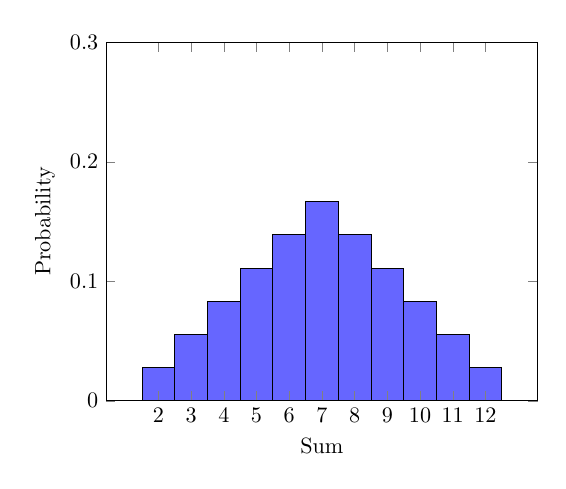
\begin{tikzpicture}[scale=0.8]
\begin{axis}[
ymin = 0, ymax = 0.3, area style, xlabel = {Sum}, ylabel = {Probability},
xtick = {2,3,...,12}
]
\addplot[ybar interval, fill=blue!60, mark=no] plot coordinates {
	(1.5,1/36) (2.5,1/18) (3.5,1/12) (4.5,1/9) (5.5,5/36) (6.5,1/6) (7.5,5/36) (8.5,1/9) (9.5,1/12) (10.5,1/18) (11.5,1/36) (12.5,1/36)
};
\end{axis}
\end{tikzpicture}
\end{center}
\end{frame}

\begin{frame}{Example 1}
(a) \quad Create a probability distribution for flipping a coin three times, where $X$ represents the number of times heads is flipped.	\newline\\	\pause

The sample space is HHH, HHT, HTH, HTT, THH, THT, TTH, and TTT	\pause

\begin{center}
\setlength{\extrarowheight}{4pt}
\begin{tabular}{c|c}
$\bm{x}$ & $\bm{P(X=x)}$ \\ \hline
0 & \onslide<4->{1/8} \\[4pt]
1 & \onslide<5->{1/4} \\[4pt]
2 & \onslide<6->{1/4} \\[4pt]
3 & \onslide<7->{1/8}
\end{tabular}
\end{center}
\end{frame}

\begin{frame}{Example 1}
(b) \quad Create a probability distribution histogram for the number of times heads appears when flipping a coin 3 times.	\newline\\	\pause

\begin{center}
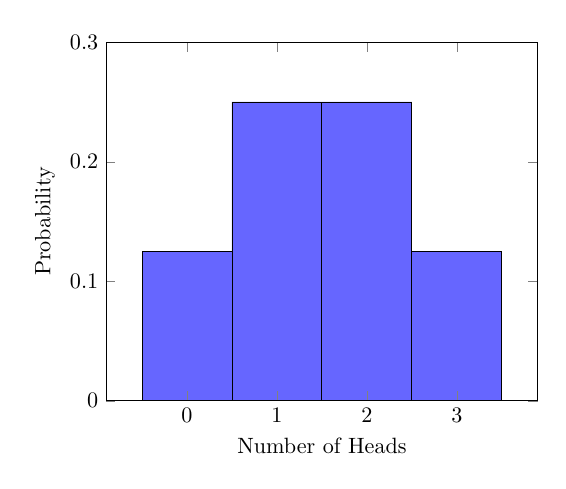
\begin{tikzpicture}[scale=0.8]
\begin{axis}[
ymin = 0, ymax = 0.3, area style, xlabel = {Number of Heads}, ylabel = {Probability},
xtick = {0,1,2,3}
]
\addplot[ybar interval, fill=blue!60, mark=no] plot coordinates {
	(-0.5,1/8) (0.5,1/4) (1.5,1/4) (2.5,1/8) (3.5,1/8)
};
\end{axis}
\end{tikzpicture}
\end{center}
\end{frame}

\begin{frame}{Example 2}
The distribution below represents the percentage of households that have $x$ dogs according to a recent study. \newline
\begin{center}
\begin{tabular}{c|c}
$\bm{x}$ & $\bm{P(X=x)}$ \\ \hline
0 & 44\% \\
1 & 27\% \\
2 & 18\% \\
3 or more & 11\%
\end{tabular}
\end{center}
How many households have at least 1 dog?	\newline\\	\pause
Using the Complement Rule: $100\% - 44\% = 56\%$
\end{frame}

\section{Determine the expected value of a probability distribution}

\begin{frame}{Expected Value}
\begin{tcolorbox}[colframe=green!20!black, colback = green!30!white,title=\textbf{Expected Value}]
The \textbf{expected value} of a probability distribution is the outcome we would expect to happen if the experiment was performed a very large number of times.
\end{tcolorbox}
\vspace{10pt} \pause

In other words, it is a {\color{blue}\textbf{weighted mean}} of the distribution of outcomes:	\newline\\
\[E(X) = \sum \left(x \cdot P(x)\right) \]
\end{frame}

\begin{frame}{Example 3}
Determine the expected value of rolling two dice.	\pause

\begin{center}
\begin{minipage}{0.4\textwidth}
\setlength{\extrarowheight}{4pt}
\begin{tabular}{c|c|c}
$x$ &  $\bm{P(X=x)}$ 	&	$x \cdot P(x)$ 	\\ \hline
2 & $\sfrac{1}{36}$ 	&  	$\sfrac{1}{18}$	\\[4pt]
3 & $\sfrac{1}{18}$ 	&	$\sfrac{1}{6}$	\\[4pt]
4 & $\sfrac{1}{12}$		&	$\sfrac{1}{3}$ 	\\[4pt]
5 & $\sfrac{1}{9}$		&	$\sfrac{5}{9}$ 	\\[4pt]
6 & $\sfrac{5}{36}$		&	$\sfrac{5}{6}$ 	\\
\end{tabular}
\end{minipage}
\hspace{8pt}
\begin{minipage}{0.4\textwidth}
\setlength{\extrarowheight}{4pt}
\begin{tabular}{c|c|c}
$x$ &  $\bm{P(X=x)}$ 	&	$x \cdot P(x)$ 	\\ \hline
7 & $\sfrac{1}{6}$ 		&	$\sfrac{7}{6}$	\\[4pt]
8 & $\sfrac{5}{36}$		&	$\sfrac{10}{9}$ \\[4pt]
9 & $\sfrac{1}{9}$		&	$1$ \\[4pt]
10 & $\sfrac{1}{12}$ 	&	$\sfrac{5}{6}$\\[4pt]
11 & $\sfrac{1}{18}$	&	$\sfrac{11}{18}$ \\[4pt]
12 & $\sfrac{1}{36}$ 	&	$\sfrac{1}{3}$
\end{tabular}
\end{minipage}
\end{center}
\end{frame}

\begin{frame}{Example 3}
The expected value is the sum of all of the entries in the last column:	\pause

\[\frac{1}{18} + \frac{1}{6} + \frac{1}{3} + \cdots + \frac{11}{18} + \frac{1}{3} = 7\]	\bigskip

Calculating the weighted mean of our distribution, the expected value of rolling two dice is 7.
\end{frame}


\begin{frame}{Example 4}
The distribution below represents the percentage of households that have $x$ dogs according to a recent study. \newline
\begin{center}
\begin{tabular}{c|c}
$\bm{x}$ & $\bm{P(X=x)}$ \\ \hline
0 & 44\% \\
1 & 27\% \\
2 & 18\% \\
3 & 11\%
\end{tabular}
\end{center}
What is the expected number of dogs per household?	\newline\\
\onslide<2->{$0(0.44) + 1(0.27) + 2(0.18) + 3(0.11) \onslide<3->{= 0.96}$}	\newline\\
\onslide<4->{There is about 1 dog per household.}
\end{frame}

\section{Determine the variance and standard deviation of a probability distribution}

\begin{frame}{Variance and Standard Deviation}
Previously, we saw that variance, which was the average squared deviation the data values are from the mean, was
\[\frac{\sum \left(x-\mu\right)^2}{n}\]
\pause

Similarly, the variance for probability distributions is given as
\[\sigma^2 = \sum\left((x-\mu)^2 \cdot P(x)\right)\]	\pause
from which the {\color{blue}\textbf{standard deviation}} is 
\[\sigma = \sqrt{\sum\left((x-\mu)^2 \cdot P(x)\right)}\]
\end{frame}

\begin{frame}{Variance and Standard Deviation Alternate Definition}
\[\sigma^2 = \sum\left((x-E(x))^2 \cdot P(x)\right)\]	\pause
and
\[\sigma = \sqrt{\sum\left((x-E(x))^2 \cdot P(x)\right)}\]
\end{frame}


\begin{frame}{Example 5}
What is the standard deviation of rolling two dice?	\newline\\	\pause

From a previous example, we have $\mu = E(x) = 7$.	\newline\\	\pause

2: \quad $(2-7)^2 \cdot \frac{1}{36} = \frac{25}{36}$	\newline\\	\pause
3: \quad $(3-7)^2 \cdot \frac{1}{18} = \frac{8}{9}$ \newline\\ \pause
$\vdots$ \newline\\ \pause
12: \quad $(12-7)^2 \cdot \frac{1}{36} = \frac{25}{36}$
\end{frame}

\begin{frame}{Example 5}
Adding up all of the results and then taking the square root, we get
\[\sigma \approx 2.415\]
\end{frame}
\end{document}